\documentclass[twoside,11pt]{article}\usepackage{amsmath,amsfonts,amsthm,fullpage}
\usepackage{amsmath}
\usepackage{amssymb}
\setlength{\parindent}{0pt}
\usepackage{graphicx}
\usepackage{bm}
\def\argmin{\operatornamewithlimits{arg\, min}}
\newcommand{\rbr}[1]{\left(#1\right)}
\newcommand{\cbr}[1]{\left\{#1\right\}}
\newcommand{\Ncal}{\mathcal{N}}
\begin{document}

\title{CS 7641 CSE/ISYE 6740 Homework 4}
\author{Bhatia Parminder}
\date{Deadline: 11/27 Thursday, 11:55 pm}
\maketitle

\begin{itemize}
  \item Submit your answers as an electronic copy on T-square.
  \item No unapproved extension of deadline is allowed. Late
  submission will lead to 0 credit.
  \item Typing with Latex is highly recommended. Typing with MS Word is also okay.
  If you handwrite, try to be clear as much as possible. No credit may be given to unreadable handwriting.
  \item Explicitly mention your collaborators if any. For the programming problem, it is
  absolutely not allowed to share your source code with anyone in the
  class as well as to use code from the Internet without reference.
  \item Recommended reading: PRML Section 13.2
 \end{itemize}
 

\section{Kernels [20 points]}
This problem will explore a number of kernels and non-kernels to get some more intuition for (i) what constitutes a valid kernel and (ii) see kind of functions we can implicitly define with kernels. Identify which of the followings is a valid kernel.  If it is a kernel, please write your answer explicitly as `True' and give mathematical proofs. If it is not a kernel, please write your answer explicitly as `False' and give explanations. 

 Suppose $K_1$ and $K_2$ are valid kernels (symmetric and positive definite) defined on $R^m\times R^m$.
\begin{enumerate}
\item $K(u,v) = \alpha K_1(u,v) + \beta K_2(u,v), \alpha,\beta\in R$.
We can prove that a function  L is a valid Kernel if we can show that for any vector v
\begin{equation}
v^T(L)v \geq 0
\end{equation}
Since $K_1$ is valid thus,
\begin{equation}
v^T(K_1)v \geq 0
\end{equation}
Lets assume that K is a valid kernel, thus if we can prove according to the above condition \\
\begin{equation}
v^T(K)v \geq 0
\end{equation}
since $\alpha$ and $\beta$  are constants, we can write K in terms of $K_1$ in the above equation as,
\begin{equation}
\begin{split}
v^T(\alpha K_1 +\beta K_2)v \\
v^T(\alpha K_1)v +v^T(\beta K_2)v \\
\alpha( v^T(K_1)v) +\beta (v^T( K_2)v) \\
\end{split}
\end{equation}
Now, since $ ( v^T(K_1)v)  \geq 0$ and we know that $\alpha$ and $\beta$ are real numbers, thus lets say for negative  $\alpha$ and $\beta$  the above equation can be less than zero. Hence, it is not a valid Kernel
\item $K(u,v) = u^\top C v$ where $C\in R^{m\times m}$.
\\Solution: False
\\\\ In this case each entry of the gram matrix is defined as $ u^\top C v $. Now, taking C to be a negative Identity matrix, lets take every element(data point) consisting of positive coefficients. Thus in every vector u ,v all coefficients are positive .  Thus,we have product matrix $u^\top C$ as negative.\\\\Further taking v to be a matrix with positive coefficients, $u^\top C v $ is matrix whose terms are negative. 
\\\\ Thus we have a gram-matrix whose all terms are negative. Thus in this case, for a vector v with positive coefficients, 
\begin{equation}
v^t K v < 0
\end{equation} 
\\\\which violates the property.
\\Thus we have shown that for particular values of matrices, the above kernel violates the property and hence is not  a valid kernel. 

\item $K(u,v) = K_1(f(u), f(v))$ where $f:R^m \rightarrow R^m$.
\\ Solution: True
\\\\ Here $K_1$ is a valid kernel defined on $R^m\times R^m$ which implies it is symmetric and positive definite
\\ Further $f:R^m \rightarrow R^m$, which is basically a mapping from real number to a real number.
Thus, we get \\
\begin{equation} \nonumber
\begin{split}
f(u) = \mu \\\\ f(v) = \gamma 
\end{split}
\end{equation}
\\\\ where $\mu$ , $\gamma \in R^m$
\\\\ Thus the expression reduces to,  $ K_1 ( \mu , \gamma ) $,which is a kernel  and thus $K(u,v) $ is a valid kernel.
\\\\

\item $K(u,v) = f(K_1(u,v))$ where $f$ is any polynomial with positive coefficients.
\\ Solution: True.
\\\\ Let $(K_1(u,v))$, can be expressed as:
\begin{equation} \nonumber
f(K_1(u,v)) = \alpha((K_1(u,v))) + \beta{(K_1(u,v))}^2 +\gamma {(K_1(u,v))}^2  + ....
\end{equation}, where coefficients are positive. \\
\\To prove the above part , we have to prove 2 parts \\
\\\\ Firstly, we have to prove that multiplication of two kernels gives a valid kernel: \\\\
Let $ K_p (x,y) = K_1(x,y) K_2(x,y) $
\\\\ Suppose $\Phi_1$ is a an M-dimensional vector, $ \Gamma_1$ is an N-dimensional vector
\begin{equation} \nonumber
\begin{split}
 K_p (x,y)= ({\Phi_1(x)}^T{\Phi_1(y)})({\Gamma_1(x)}^T{\Gamma_1(y)}) \\\\
= (\sum_{m=1}^M \Phi_m(x)\Phi_m(y))(\sum_{n=1}^{N} \Gamma_n(x)\Gamma_n(y))\\\\
= \sum_{m=1}^M \sum_{n=1}^N \Phi_m(x)\Phi_m(y) \Gamma_n(x)\Gamma_n(y)\\\\
= \sum_{m=1}^M \sum_{n=1}^N (\Phi_m(x)\Gamma_n(x))(\Phi_m(y)\Gamma_n(y)) \\\\
= c(x)^T c(y) 
\end{split}
\end{equation}
\\\\ where $c(x)$ is M.N dimensional vector.
\\\\ Thus it can be seen that, product of two kernels is a valid kernel.  \\[.25cm]
Second part we have to prove  that linear summation of two kernels is also a kernel, given that coefficients are non-negative.\\
\\ $ K(u,v) = {\Phi(u)}^T{\Phi(v)}$
\\\\Assuming both $\alpha$ and $\beta$ can be factored as a multiplication of their roots, both the given kernels $K_1$, $K_2$ can be expressed as
\begin{equation} \nonumber
\begin{split}
K_1(u,v) &= {\sqrt{\alpha}\Phi_1(u)}^T{\sqrt{\alpha}\Phi_1(v)} \\
K_2(u,v) &= {\sqrt{\beta}\Phi_1(u)}^T{\sqrt{\beta}\Phi_1(v)}
\end{split}
\end{equation}
\\\\ Thus $K(u,v) $ can be written as,
\begin{equation} \nonumber
\begin{split}
K(u,v) = ({\sqrt{\alpha}\Phi_1(u)}^T{\sqrt{\alpha}\Phi_1(v)}) +  ({\sqrt{\beta}\Phi_1(u)}^T{\sqrt{\beta}\Phi_1(v)})   \\\\
K(u,v) = {[\sqrt{\alpha}\Phi_1(u) \sqrt{\beta}\Phi_1(u)]}^T [\sqrt{\alpha}\Phi_1(v)   \sqrt{\beta}\Phi_1(v)]
\end{split}
\end{equation}
\\\\ Now since $\alpha$ and $\beta$ are positive valued, their roots can be real. Hence K(u,v) is  a valid kernel. 
Thus,  $K(u,v) = f(K_1(u,v))$ is a valid kernel.\\
\item $K(u,v) = \exp{K_1(u,v)}$.

Solution: True. 
\\\\ \begin{equation} \nonumber
exp(x)  = lim_{(n \rightarrow \infty)} (1 + x + \frac{x^2}{2!} + ...... \frac{x^n}{n!})
\end{equation}
\\\\ As explained in the last solution, each term is a product of kernel and hence a valid kernel. Further since the coefficients are positive, it represents a valid kernel.\\\\

\item \begin{align}
	K(u,v) = \left\{
	\begin{aligned}
	&1 & \text{if } \|u-v\|_2 \leqslant 1\\
	& 0 & \text{otherwise}
	\end{aligned}
	\right.
	\end{align}
	\\Solution: False
\\\\ K(u,v) would be a square matrix whose all diagonal elements are definitely 1 while all other elements can b either 0 or 1.
\\ We assume K(u,v) to be a square matrix of size 2, with diagonal elements as 1, and other elements as a and b. $ a, b \in (0,1) $
\\\\ For K to be a valid kernel, for any given vector v, 
\begin{equation} \nonumber
v^T K v \geq 0
\end{equation}
Thus, we assume v = [a   b   c]
\begin{equation} \nonumber
\begin{bmatrix}
a & b & c\\
\end{bmatrix}
\begin{bmatrix}
1 & 1 & 1 \\
1 & 1 & 0\\
1 & 0 & 1\\
\end{bmatrix}
\begin{bmatrix}
a \\
b \\
c \\
\end{bmatrix} \geq 0 
\end{equation}
\begin{equation} \nonumber
(a+b)^2 + 2ac + c^2 \geq 0  \\\\
\end{equation}
 For following values, a = -1, b = 0.5,  c = 1, the above equation evaluates to negative
Hence K is not a valid kernel.
\\\\
	

\item Suppose $K'$ is a valid kernel. 
	\begin{align}
	K(u,v) = \frac{K'(u,v)}{\sqrt{K'(u,u)K'(v,v)}}.
	\end{align}
Solution :True \\
The meaning of the above equation is that we can normalize the data in feature space without performing  explicit mapping. \\
\begin{equation}
\begin{split}
	K(u,v) = \frac{K'(u,v)}{\sqrt{K'(u,u)K'(v,v)}}\\
	= \frac{({\Phi_1(u)}^T{\Phi_1(v)})}{\sqrt{||u||^2 ||v||^2}}\\
	= ({\Phi_1(\frac{u}{||u||^2})}^T{\Phi_1(\frac{v}{||v||^2})})\\
\end{split}
\end{equation}
\end{enumerate} 
 
 

\section{Markov Random Field, Conditional Random Field [20 pts]}

\textbf{[a-b]} A probability distribution on  3 discrete variables
a,b,c is defined by $P(a,b,c) = \frac{1}{Z}\psi(a,b,c) =
\frac{1}{Z}\phi_1(a,b)\phi_2(b,c)$, where the table for the two
factors are given below.

\begin{table}[!htb]

    \begin{minipage}{.5\linewidth}

      \centering

    \begin{tabular}{cc|c}
    a & b & $\phi_1(a,b)$ \\ \hline
    0 & 0 & 4             \\
    0 & 1 & 2             \\
    1 & 0 & 3             \\
    1 & 1 & 1             \\
    \end{tabular}

    \end{minipage}%
    \begin{minipage}{.5\linewidth}
      \centering
     \begin{tabular}{cc|c}
    b & c & $\phi_2(b,c)$ \\ \hline
    0 & 0 & 2             \\
    0 & 1 & 2             \\
    0 & 2 & 1             \\
    1 & 0 & 4             \\
    1 & 1 & 1             \\
    1 & 2 & 2             \\
    \end{tabular}
    \end{minipage}
\end{table}

\subsubsection*{(a) Compute the slice of the joint factor $\psi(a,b,c)$ corresponding to $b = 1$. This is the table $\psi(a,b=1,c)$. [5 pts]}
To compute $\psi(a,b=1,c)$ , we need to calculate for all values of a and c given the value of b .
Thus,
\begin{equation}
\psi(a,b=1,c) = \psi(0,1,0) + \psi(0,1,1)+ \psi(0,1,2)+ \psi(1,1,0)+ \psi(1,1,1)+ \psi(0,1,2)
\end{equation}
Now 
\begin{equation}
\psi(0,1,0) = \phi_1(0,1)\phi_2(1,0) = 2*4=8
\end{equation}
Similarly
\begin{equation}
\begin{split}
\psi(0,1,1) =  2*1=2\\
\psi(0,1,2) =  4\
\psi(1,1,0) =  4\\
\psi(1,1,1) =  1\\
\psi(1,1,2) =  2\\
\end{split}
\end{equation}
Summing all the values we get
\begin{equation}
\psi(a,b=1,c) = 8+2+4+4+1+2=21
\end{equation}
\subsubsection*{(b) Compute $P(a = 1,b = 1)$. [5 pts]}
To compute the probability we need to find the constant Z, which is basically sum of all the iterations.

\begin{equation}
\begin{split}
\psi(0,1,0) = \phi_1(0,1)\phi_2(1,0) = 2*4=8\\
\psi(0,1,1) =  2*1=2\\
\psi(0,0,0) =  8\\
\psi(0,1,1) =  2\\
\psi(0,1,2) =  4\\
\psi(0,0,2) =  4\\
\psi(1,1,0) = 4\\
\psi(1,1,1) = 1\\
\psi(1,0,0) =  6\\
\psi(1,1,1) =  1\\
\psi(1,1,2) =  2\\
\psi(1,0,2) =  3\\
\end{split}
\end{equation}

\begin{equation}
\begin{split}
Z = \sum \psi(a,b,c) =56
\end{split}
\end{equation}
Now $P(a = 1,b = 1)$ is given by
\begin{equation}
\begin{split}
P(a = 1,b = 1 = \frac{\psi(1,1,0) + \psi(1,1,1)+ \psi(1,1,2)}{Z}\\
=7/56
\end{split}
\end{equation}
%\newpage

\iffalse
\textbf{[c-d]} Consider a probability distribution $P$ over four
binary variables $X_1$, $X_2$, $X_3$, and $X_4$ as below. The
distribution assigns probability $1/8$ to each of the following
configurations, and the probability 0 to all others. Let $H$ be an
undirected graph $X_1$--$X_2$--$X_3$--$X_4$--$X_1$.

\begin{table}[!h]
     \centering
    \begin{tabular}{cccc|c}
    \hline
    $X_1$ & $X_2$ & $X_3$   & $X_4$ & P   \\ \hline
    0     & 0     & 0       & 0     & 1/8 \\
    0     & 0     & 0       & 1     & 1/8 \\
    1     & 0     & 0       & 0     & 1/8 \\
    0     & 0     & 1       & 1     & 1/8 \\
    1     & 1     & 0       & 0     & 1/8 \\
    0     & 1     & 1       & 1     & 1/8 \\
    1     & 1     & 1       & 0     & 1/8 \\
    1     & 1     & 1       & 1     & 1/8 \\ \hline
    \multicolumn{4}{l|}{All other tuples}  & 0   \\ \hline
    \end{tabular}
\end{table}
\noindent

~\\
\subsubsection*{(c) Show that $P$ satisfies all of the global independencies implied by $H$. In other words, $I(H)$ is a subset of $I(P)$. [5 pts]}

\emph{Hint}: Test each independency numerically.

\subsubsection*{(d) Show that $P$ does not factorize over $H$. In other words, $P$ cannot be expressed as a product of potential functions defined over the cliques of $H$. [7 pts]}

\emph{Hint:} Use a proof by contradiction. Show that the joint
probability of a single assignment is not equal to the product of
the clique factors under that assignment.) Comment on the
consequences of allowing zero probabilities in Markov models.


~\\

\textbf{[e-f]} Let $H$ be a Markov network in variables $A, B, C, D,
E, F$, which is connected. Consider performing variable elimination,
with the elimination order $A, B, C, D, E, F$. Use the following
template to answer.

\begin{figure}[h!]
\centering
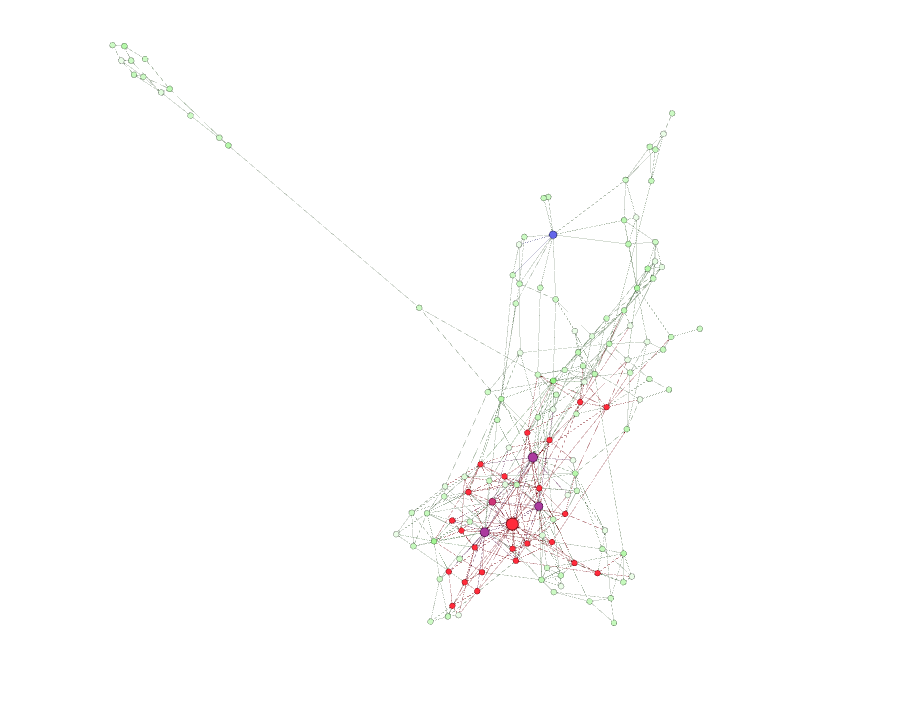
\includegraphics[width=30mm]{graph.png}
\label{overflow}
\end{figure}

\subsubsection*{(e) Draw in the missing edges for $H$ below, such that the number of fill edges added during variable
elimination is maximized. Draw the primary edges for $H$ as solid
lines, and the resulting fill edges as dashed lines. Draw the
resulting clique tree. Note that your solution for $H$ must result
in each node being connected to at least one other node.) [6 pts]}

\subsubsection*{(f) Repeat (e), so that the number of fill edges is minimized. Draw the resulting
clique tree. Note that each node must be connected to at least one
other node in $H$.) [6 pts]}

~\\
\fi

\subsubsection*{(c) Explain the difference between Conditional Random Fields and Hidden
Markov Models with respect to the following factors. Please give
only a one-line explanation. [10 pts]}

\begin{itemize}
  \item Type of model - generative/discriminative
  \\ Solution: \\\\
  HMMs are generative classifiers while CRFs are discriminative classifier models. HMM try to find the label using the joint probability of label with data, where as CRFs directly go for the decision boundary ,given the data. HMMs are sequential extension of Naive Bayes' classifier while CRFs are that of Logistic Regression.
  \item Objective function optimized
  \\Solution:\\\\
  In generative models such as HMM, we use Bayes rule to compute the conditional likelihood of labels. Thus the objective function optimized by HMM is the joint likelihood:
\begin{equation}
\hat{y}  = arg \quad max_{y} \prod_{i=1}^n P(x,y)
  \end{equation}
\\discriminative models like CRFs optimize the conditional likelihood of the labels given the observed data directly
\begin{equation}
\hat{y} = arg \qquad max_{y} \quad log P(y/x)
\end{equation}
  \item Require a normalization constant
  \\ Solution: \\\\
To overcome the problem of label bias, i.e., influence of local distributions on the global choice of latent variables, probabilities in CRF are normalized globally. 
\\ In HMMs, one latent factor depends sequentially on the its previous M states and thus doesn't suffer from this problem. 
\\\\ Thus normalizing constants are required for CRFs only.
\end{itemize}
~\\~\\

\section{Hidden Markov Model [50 pts]}

This problem will let you get familiar with HMM algorithms by doing
the calculations by hand.

\textbf{[a-c]} There are three coins $(1,2,3)$, to throw them
randomly, and record the result. $S = {1,2,3}$; $V = {H,T}$ (Head or
Tail); $A, B, \pi$ is given as

\begin{table}[!htb]
    \begin{minipage}{.5\linewidth}
      \centering
A:
    \begin{tabular}{l|l|l|l}
    ~ & 1    & 2    & 3    \\\hline
    1 & 0.9  & 0.05 & 0.05 \\
    2 & 0.45 & 0.1  & 0.45 \\
    3 & 0.45 & 0.45 & 0.1  \\
    \end{tabular}

    \end{minipage}%
    \begin{minipage}{.5\linewidth}
      \centering

B:
    \begin{tabular}{l|l|l|l}
    ~ & 1   & 2    & 3    \\\hline
    H & 0.5 & 0.75 & 0.25 \\
    T & 0.5 & 0.25 & 0.75 \\
    \end{tabular}

    \end{minipage}

    \begin{minipage}{.5\linewidth}
      \centering
$\pi:$
    \begin{tabular}{llll}
    $\pi$ & 1/3 & 1/3 & 1/3 \\
    \end{tabular}
  \end{minipage}

\end{table}

\subsubsection*{(a) Given the model above, what's the probability of observation $O = {H,T,H}$. [5 pts]}
To calculate the probability of the observation we need to find 
\begin{equation}
P(H,T,H) = \sum P(H,T,H,Z_1,Z_2,Z_3)
\end{equation}
Thus we need to find the probability for all the sequence of coins.\\
For a given sequence, probability is defined using Hidden Markov Chain
\begin{equation}
\begin{split}
P(H,T,H,1,2,3) = P(1)*P(H/1)*P(2/1)*P(T/2)*P(3/2)*P(H/3)\\
(.33)(.5)(.05)(.25)(.45)(.25) = .00023
\end{split}
\end{equation}
Similarly , we can find the other probabilities as :
\begin{equation}
\begin{split}
P(H,T,H,1,3,2) = P(1)*P(H/1)*P(3/1)*P(T/3)*P(2/3)*P(H/2)=(.33)(.5)(.05)(.75)(.45)(.75) = .00211 \\
P(H,T,H,3,2,1) =(.33)(.25)(.45)(.25)(.45)(.5) = .00211 \\
\end{split}
\end{equation}
Similarly, I used code to get the following results:\\
1,1,1 : 0.03375\\
1,1,2 : 0.0028125000000000003\\
1,1,3 : 9.375000000000001E-4\\
1,2,1 : 4.6875000000000004E-4\\
1,2,2 : 1.5625000000000003E-4\\
1,2,3 : 2.3437500000000002E-4\\
1,3,1 : 0.0014062500000000004\\
1,3,2 : 0.002109375\\
1,3,3 : 1.5625000000000003E-4\\
2,1,1 : 0.0253125\\
2,1,2 : 0.002109375\\
2,1,3 : 7.031250000000001E-4\\
2,2,1 : 0.0014062500000000004\\
2,2,2 : 4.6875000000000004E-4\\
2,2,3 : 7.031250000000002E-4\\
2,3,1 : 0.018984375\\
2,3,2 : 0.0284765625\\
2,3,3 : 0.002109375\\
3,1,1 : 0.0084375\\
3,1,2 : 7.031250000000001E-4\\
3,1,3 : 2.3437500000000002E-4\\
3,2,1 : 0.002109375\\
3,2,2 : 7.031250000000001E-4\\
3,2,3 : 0.0010546875\\
3,3,1 : 0.0014062500000000004\\
3,3,2 : 0.002109375\\
3,3,3 : 1.5625000000000003E-4\\
Total Probablility::0.13921875\\
Max Probablility Sequence::1 1 1
Thus , probability of observation $O = {H,T,H}$ is the sum of all, which is equal to $0.13921875$\\
\subsubsection*{(b) Given the observation, what's the most likely sequence (the number of coin), how do you get the result? [5 pts]}
Most likely sequence is (1,1,1). \\ Basically, we have to find $P(Z_1,Z_2,Z_3/ data)$ . \\
From the above part , we found the joint probability given by $P(H,T,H,Z_1,Z_2,Z_3)$, thus we can find the conditional probability using the Bayes equation.
\begin{equation}
\begin{split}
P(Z_1,Z_2,Z_3/ data)= P(H,T,H,Z_1,Z_2,Z_3)/P(H,T,H)\\
\end{split}
\end{equation}
Note that probability for any data sequence can be assumed to be equal (1/27). Thus conditional probability is governed by the joint probability, which is maximum for sequence (1,1,1) , as calculated in the first part.\\

\subsubsection*{(c) Describe how to get the $A, B$, and $\pi$, when they are unknown. [10 pts]} 

Let us consider discrete HMMs of length $T$ (each observation sequence is $T$ observations long). Let the space of observations be $X = \{1, 2, \ldots , N\}$, and let the space of underlying states be $Z = \{1, 2, \dots , M\}$. An HMM $\theta = (\pi, A, B)$ is parameterized by the initial state matrix $\pi$, the state transition matrix $A$, and the emission matrix $B$. Here, $\pi_i = P(z_i)$, $A_{ij} = P(z_{t+1} = j | z_t = 1)$, and $B_{i}(j) = P(x_t = j | z_t = i)$. \\

We study the problem of learning the parameterization of $\theta$ from a dataset of $D$ observations. Let $X = X^{(1)}, \ldots , X^{(D)}$, where each $X^{(i)} = (x^{(i)}_1, \ldots, x^{(i)}_T)$. We assume each observation is drawn iid. The learning problem is nontrivial because we are not given the latent variables $Z^{(i)}$ for each $X^{(i)}$. Thus, we will directly compute $\theta^* = argmax_{\theta} \sum_{z \in Z} P(X , z; \theta)$. \\

Baum-Welch is an iterative procedure for estimating $\theta^*$ from only $X$ . It works by maximizing the log-likelihood, and updating the current model to be closer to the optimal model. Each iteration of Baum-Welch is guaranteed to increase the log-likelihood of the data. But of course, convergence to the optimal solution is not guaranteed. \\

Baum-Welch can be described simply as repeating the following steps until convergence:

\begin{itemize}
\item Compute $Q(\theta, \theta^s) = \sum_{z \in Z} \log [P(X , z; \theta)] P(z | X ; \theta^s)$.
\item Set $\theta^{s+1} = argmax_{\theta}\ Q(\theta, \theta^s)$.
\end{itemize}

First, we note that $P(z, X ) = P(X )P(z|X )$. Thus, we can write:

\begin{equation} \nonumber
\begin{split}
argmax_{\theta} \sum_{z \in Z} \log [P(X , z; \theta)] P(z|X ; \theta^s) &= argmax_\theta \sum_{z \in Z} \log [P(X , z; \theta)] P(z, X ; \theta^s) \\
&= argmax_{\theta} \hat{Q}(\theta, \theta^s)
\end{split}
\end{equation}

Since $P(X)$ is not affected by choice of $\theta$. Now $P(z, X ; \theta)$ is easy to write down as:

\begin{equation} \nonumber
\begin{split}
P(z, X ; \theta) &= \prod^D_{d=1} \left( \pi_{z_1^{(d)}} B_{z_1^{(d)}} (x_1^{(d)}) \prod^T_{t=2} A_{{z_{t-1}^{(d)}}{z_{t}^{(d)}}} B_{z_t^{(d)}} (x_t^{(d)}) \right)
\end{split}
\end{equation}

Taking the log, we get

\begin{equation} \nonumber
\log P(z, X ; \theta) = \sum^D_{d=1} \left[ \log \pi_{z_1^{(d)}} + \sum^T_{t=2} \log A_{{z_{t-1}^{(d)}}{z_{t}^{(d)}}} + \sum^T_{t=1} \log B_{z_t^{(d)}} (x_t^{(d)}) \right]
\end{equation}

Plugging this into $\hat{Q}(\theta, \theta^s)$, we get:

\begin{equation} \nonumber
\begin{split}
\hat{Q}(\theta, \theta^s) = \sum_{z \in Z} \sum^D_{d=1} \log \pi_{z_1^{(d)}} P(z, X ; \theta^s) + \sum_{z \in Z} \sum^D_{d=1} \sum^T_{t=2} \log A_{{z_{t-1}^{(d)}}{z_{t}^{(d)}}} P(z, X ; \theta^s) + \sum_{z \in Z} \sum^D_{d=1} \sum^T_{t=1} \log B_{z_t^{(d)}} (x_t^{(d)})  P(z, X ; \theta^s)
\end{split}
\end{equation}

This is a nice form which we can optimize analytically with Lagrange multipliers. We need Lagrange multipliers
because we have equality constraints which come from requiring that $\pi$, $A_{i.}$ and $B_{i(.)}$ form valid probability distributions. \\

Let $\hat{L}(\theta, \theta^s)$ be the Lagrangian,

\begin{equation} \nonumber
\begin{split}
\hat{L}(\theta, \theta^s) = \hat{Q}(\theta, \theta^s) - \lambda_{\pi} \left( \sum^M_{i=1} \pi_i - 1 \right) - \sum^M_{i=1} \lambda_{A_i} \left( \sum^M_{j=1} A_{ij} - 1 \right) - \sum^M_{i=1} \lambda_{B_i} \left( \sum^N_{j=1} B_{i}(j) - 1 \right)
\end{split}
\end{equation}

For $\pi_i$, we get:

\begin{equation} \nonumber
\begin{split}
\frac{\partial \hat{L}(\theta, \theta^s)}{ \partial \pi_i} &= \frac{\partial}{ \partial \pi_i} \left( \sum_{z \in Z} \sum^D_{d=1} \log \pi_{z_1^{(d)}} P(z, X ; \theta^s) \right) - \lambda_{\pi} = 0 \\
&= \frac{\partial}{ \partial \pi_i} \left( \sum^M_{j=1} \sum^D_{d=1} \log \pi_{j} P(z_1^{(d)} = j, X ; \theta^s) \right) - \lambda_{\pi} = 0 \\
&= \sum^D_{d=1} \frac{P(z_1^{(d)} = i, X ; \theta^s)}{\pi_i} = 0 \\
\frac{\partial \hat{L}(\theta, \theta^s)}{ \partial \lambda_{\pi}} &= - \left( \sum^M_{i=1} \pi_i - 1 \right) = 0
\end{split}
\end{equation}

The second step is simply the result of marginalizing out, for each $d$, all $z_{t \neq 1}^{(d)}$ and $z_t^{(d^t \neq d)}$ for all $t$. We get:

\begin{equation} \nonumber
\begin{split}
\pi_i &= \frac{\sum^D_{d=1} P(z_1^{(d)} = i, X ; \theta^s)}{\sum^M_{j=1} \sum^D_{d=1} P(z_1^{(d)} = j, X ; \theta^s)} = \frac{\sum^D_{d=1} P(z_1^{(d)} = i, X ; \theta^s)}{\sum^D_{d=1} \sum^M_{j=1}  P(z_1^{(d)} = j, X ; \theta^s)} \\
&= \frac{\sum^D_{d=1} P(z_1^{(d)} = i, X ; \theta^s)}{\sum^D_{d=1} P(X ; \theta^s)} = \frac{\sum^D_{d=1} P(z_1^{(d)} = i, X ; \theta^s)}{D\ P(X ; \theta^s)} \\
&= \frac{\sum^D_{d=1} P(X ; \theta^s) P(z_1^{(d)} = i | X ; \theta^s)}{D\ P(X ; \theta^s)} = \frac{1}{D} \sum^D_{d=1} P(z_1^{(d)} = i | X ; \theta^s) \\
&= \frac{1}{D} \sum^D_{d=1} P(z_1^{(d)} = i | X^{(d)} ; \theta^s)
\end{split}
\end{equation}

For the $A_{ij}$, we get:

\begin{equation} \nonumber
\begin{split}
\frac{\partial \hat{L}(\theta, \theta^s)}{ \partial A_{ij}} &= \frac{\partial}{ \partial A_{ij}} \left( \sum_{z \in Z} \sum^D_{d=1} \sum^T_{t=2} \log A_{{z_{t-1}^{(d)}}{z_{t}^{(d)}}} P(z, X ; \theta^s)  \right) - \lambda_{A_{ij}} = 0 \\
&= \frac{\partial}{ \partial A_{ij}} \left( \sum_{j=1}^M \sum_{k=1}^M \sum^D_{d=1} \sum^T_{t=2} \log A_{jk} P({z_{t-1}^{(d)}} = j,  {z_{t}^{(d)}} = k, X ; \theta^s)  \right) - \lambda_{A_{ij}} = 0 \\
&= \sum^D_{d=1} \sum^T_{t=2} \frac{P({z_{t-1}^{(d)}} = i,  {z_{t}^{(d)}} = j, X ; \theta^s)}{A_{ij}} - \lambda_{A_{ij}} = 0 \\
\frac{\partial \hat{L}(\theta, \theta^s)}{ \partial \lambda_{A_{ij}}} &= - \left( \sum^M_{j=1} A_{ij} - 1 \right) = 0
\end{split}
\end{equation}

This yields:

\begin{equation} \nonumber
\begin{split}
A_{ij} &= \frac{\sum^D_{d=1} \sum^T_{t=2} P({z_{t-1}^{(d)}} = i,  {z_{t}^{(d)}} = j, X ; \theta^s)}{ \sum_M^{j=1} \sum^D_{d=1} \sum^T_{t=2} P({z_{t-1}^{(d)}} = i,  {z_{t}^{(d)}} = j, X ; \theta^s)} \\
&= \frac{\sum^D_{d=1} \sum^T_{t=2} P({z_{t-1}^{(d)}} = i,  {z_{t}^{(d)}} = j, X ; \theta^s)}{ \sum^D_{d=1} \sum^T_{t=2} P({z_{t-1}^{(d)}} = i, X ; \theta^s)} \\
&= \frac{\sum^D_{d=1} \sum^T_{t=2} P(X ; \theta^s) P({z_{t-1}^{(d)}} = i,  {z_{t}^{(d)}} = j | X ; \theta^s)}{ \sum^D_{d=1} \sum^T_{t=2} P(X ; \theta^s) P({z_{t-1}^{(d)}} = i | X ; \theta^s)} \\
&= \frac{\sum^D_{d=1} \sum^T_{t=2} P({z_{t-1}^{(d)}} = i,  {z_{t}^{(d)}} = j | X^{(d)} ; \theta^s)}{ \sum^D_{d=1} \sum^T_{t=2} P({z_{t-1}^{(d)}} = i | X^{(d)} ; \theta^s)} \\
\end{split}
\end{equation}

For $B_{i}(j)$, we will do the following:
Let $I(x)$ denote an indicator function which is 1 if $x$ is true, 0 otherwise.

\begin{equation} \nonumber
\begin{split}
\frac{\partial \hat{L}(\theta, \theta^s)}{ \partial B_{i}(j)} &= \frac{\partial}{ \partial B_{i}(j)} \left(  \sum_{z \in Z} \sum^D_{d=1} \sum^T_{t=1} \log B_{z_t^{(d)}} (x_t^{(d)})  P(z, X ; \theta^s)  \right) - \lambda_{B_{i}(j)} = 0 \\
&= \frac{\partial}{ \partial B_{i}(j)} \left(  \sum_{i=1}^N \sum^D_{d=1} \sum^T_{t=1} \log B_{i} (x_t^{(d)})  P(z_t^{(d)} = i, X ; \theta^s)  \right) - \lambda_{B_{i}(j)} = 0 \\
&= \sum^D_{d=1} \sum^T_{t=2} \frac{P({z_{t}^{(d)}} = i, X ; \theta^s) I(x_t^{(d)} = j)}{B_{i}(j)} - \lambda_{B_{i}(j)} = 0 \\
\frac{\partial \hat{L}(\theta, \theta^s)}{ \partial \lambda_{B_{i}(j)}} &= - \left( \sum^N_{j=1} B_{i}(j) - 1 \right) = 0
\end{split}
\end{equation}

From this, we get:

\begin{equation} \nonumber
\begin{split}
B_{i}(j) &= \frac{\sum^D_{d=1} \sum^T_{t=1} P({z_{t}^{(d)}} = i, X ; \theta^s) I(x_t^{(d)} = j)}{ \sum_{i=1}^N \sum^D_{d=1} \sum^T_{t=1} P({z_{t}^{(d)}} = i, X ; \theta^s) I(x_t^{(d)} = j)} \\
&= \frac{\sum^D_{d=1} \sum^T_{t=1} P({z_{t}^{(d)}} = i, X ; \theta^s) I(x_t^{(d)} = j)}{ \sum^D_{d=1} \sum^T_{t=1} P({z_{t}^{(d)}} = i, X ; \theta^s)} \\
&= \frac{\sum^D_{d=1} \sum^T_{t=1} P({z_{t}^{(d)}} = i | X^{(d)} ; \theta^s) I(x_t^{(d)} = j)}{ \sum^D_{d=1} \sum^T_{t=1} P({z_{t}^{(d)}} = i | X^{(d)} ; \theta^s)}
\end{split}
\end{equation}

Thus, we get:

\begin{equation} \nonumber
\begin{split}
\pi_i^{s+1} &= \frac{1}{D} \sum^D_{d=1} P(z_1^{(d)} = i | X^{(d)} ; \theta^s) \\
A_{ij}^{s+1} &= \frac{\sum^D_{d=1} \sum^T_{t=2} P({z_{t-1}^{(d)}} = i,  {z_{t}^{(d)}} = j | X^{(d)} ; \theta^s)}{ \sum^D_{d=1} \sum^T_{t=2} P({z_{t-1}^{(d)}} = i | X^{(d)} ; \theta^s)} \\
B_{i}^{s+1}(j) &= \frac{\sum^D_{d=1} \sum^T_{t=1} P({z_{t}^{(d)}} = i | X^{(d)} ; \theta^s) I(x_t^{(d)} = j)}{ \sum^D_{d=1} \sum^T_{t=1} P({z_{t}^{(d)}} = i | X^{(d)} ; \theta^s)}
\end{split}
\end{equation}

\subsubsection*{(d) In class, we studied discrete HMMs with discrete hidden states and
observations. The following problem considers a continuous density
HMM, which has discrete hidden states but continuous observations.
Let $S_t \in {1, 2, ..., n}$ denote the hidden state of the HMM at
time t, and let $X_t \in R$ denote the real-valued scalar
observation of the HMM at time t. In a continuous density HMM, the
emission probability must be parameterized since the random variable
$X_t$ is no longer discrete. It is defined as $P(X_t = x|S_t = i) =
\mathcal{N}(\mu_i,\sigma_i^2)$. Given $m$ sequences of observations
(each of length $T$), derive the EM algorithm for HMM with Gaussian
observation model. [14 pts]}

%Number of dimensions per observation - T (P)\\
%Number of clusters within a state - n (m)\\

Length of each sequence = T \\
No. of sequences = m \\

In the continuous case the observations at each time step $t$ are m-dimensional real-valued vectors ie $x_t = ( x_{t1}, \ldots , x_{tm} )$. \\

The EM Function is defined over all possible $S\ m$ sequences of high-level and low-level hidden states.

$$ Q(\theta, \theta^*) = \underset{S}{\sum} \underset{m}{\sum} P_\theta (S_m | x) log P_{\theta^*} (S_m,x)$$

Since,

$$ P_{\theta^*} (S_m,x) = \pi_{S_1} B_{S_1 m_1} \mathcal{N} (x_1, \mu_{S_1 m_1}, \sum_{S_1 m_1} ), \ldots , A_{S_{T-1} S_T} B_{S_t m_t} \mathcal{N} (x_T, \mu_{S_T m_T}, \sum_{S_T m_T} ) $$

Thus, it follows that,

\begin{equation} \nonumber
\begin{split}
Q(\theta, \theta^*) &= \underset{S}{\sum} \underset{m}{\sum} P_\theta(S_m | x) \log \pi_ {S_1} + \sum_{t=1}^{T-1} \sum_{S} \sum_{m} P_\theta ( S_m | x ) \log A_{S_t S_{t+1}} + \sum_{t=1}^{T} \sum_{S} \sum_{m} P_\theta ( S_m | x ) \log B_{S_t m_t} + \sum_{t=1}^{T} \sum_{S} \sum_{m} P_\theta ( S_m | x ) \log \mathcal{N} (x_t, \mu_{S_t m_t}, \sum_{S_t m_t})
\end{split}
\end{equation}

The factors in the first two terms are independent of $m$, they simplify into:

$$ \underset{S}{\sum} \underset{m}{\sum} P_\theta(S_m | x) \log \pi_ {S_1} = \sum_{S} P_{\theta}(S | x) \log \pi_{S_1} $$

and

$$ \sum_{t=1}^{T-1} \sum_{S} \sum_{m} P_\theta ( S_m | x ) \log A_{S_t S_{t+1}} = \sum_{t=1}^{T-1} \sum_{S} P_\theta (S|x) \log A_{S_t S_{t+1}}$$

The terms are identical as in the discrete case and thus applying the same training rules for initial state probabilities and for state transition probabilities apply here.\\

To find the training formulas for the cluster gains, we focus on the part of $Q(.)$ dependent on the gain terms. This part can be transformed as follows:

\begin{equation} \nonumber
\begin{split}
\sum_{t=1}^{T-1} \sum_{S} \sum_{m} P_\theta ( S_m | x) \log B_ {S_t} (m_t) &= \sum_{t=1}^{T} \sum_{i=1}^{N} \sum_{k=1}^{M} \sum_{S} \sum_{m} P_\theta ( S_m | x) \log B_{ik} \delta(i, S_t) \delta (j, m_t) \\
&= \sum_{t=1}^{T} \sum_{i=1}^{N} \sum_{k=1}^{M} P_\theta ( S_t = i, m_t = k | x) \log B_{ik}
\end{split}
\end{equation}

Thus, the part of $Q(.)$ that depends on $B_{ik}$ is of the form of $w_j \log (b_j) $ with $b_j = B_{ik}$ and 

$$ w_j = \sum_{t=1}^{T} P_\theta (S_t = i, m_t = k | x)$$

with constraints $\sum_{j} b_j = 1$ and $b_j  \le 0$ with maximum achieved for

$$  b_j = \frac{w_j} { \sum_{j} w_j }$$

Thus,

\begin{equation} \nonumber
\begin{split}
B_{ik} &= \frac{ \sum_{t=1}^{T} P_\theta(S_t = i, m_t = k | x)} { \sum_{t=1}^{T} \sum_{k=1}^{M} P_\theta ( S_t = i, m_t = k | x)} \\
&=  \frac{ \sum_{t=1}^{T} P_\theta(S_t = i, m_t = k | x)} { \sum_{t=1}^{T} P_\theta ( S_t = i | x)}
\end{split}
\end{equation}

To find the learning rules for the centroids and variances we focus on the part of $Q(.)$ that depends on the cluster centroids and variances, which is given by the following expression : 

\begin{equation} \nonumber
\begin{split}
\sum_{t=1}^{T} \sum_{S} \sum_{m} P_\theta (S_m | x) \log \mathcal{N}(x_t, \mu_{S_t m_t}, \sum_{S_t m_t}) &= \sum_{t=1}^{T} \sum_{i=1}^{N} \sum_{k=1}^{M} \sum_{S} \sum_{m} P_\theta( S_m | x) \log \mathcal{N} (x_t, \mu_{ik}, \sum_{ik}) \delta(i,S_t) \delta (k, m_t) \\
&= \sum_{t=1}^{T} \sum_{i=1}^{N} \sum_{k=1}^{M}  P_\theta (S_t = i, m_t = k | x) \log \mathcal{N} (x_t, \mu_{ik}, \sum_{ik})
\end{split}
\end{equation}

To maximize, differentiating with respect to $ \mu_{ikn} $ and equating to 0. 

\begin{equation} \nonumber
\begin{split}
\frac{\partial}{\partial \mu_{ikn}}\sum_{t=1}^{T} \sum_{i=1}^{N} \sum_{k=1}^{M}  P_\theta (S_t = i, m_t = k | x) \log \mathcal{N} (x_t, \mu_{ik}, \sum_{ik}) = 0
\end{split}
\end{equation}

Now, since,

$$ \frac{\partial \log \mathcal{N} (x_t,  \mu_{ik}, \sum_{ik} )}{\partial \mu_{ikn}} = \frac{1}{ \sigma_{ikl}^2}(x_{tl} -\mu_{ikn})$$

Thus, it follows that at a maximum,

\begin{equation} \nonumber
\begin{split}
\sum_{t=1}^{T} P_\theta(S_t = i, m_T = k | x)(x_{tl} - \mu_{ikn}) &= 0 \\
\mu_{ikn} &= \frac {\sum_{t=1}^{T} P_\theta (q_t =i m_t = k | o) o_{tn}} {\sum_{t=1}^{T} P_\theta(q_t=i | o)}
\end{split}
\end{equation}

A similar argument can be made for the diagonal variance $\sigma_{ikl}^{2}$ In this case,

$$ \frac{\partial \log \mathcal{N} (x_t, \mu_{ik}, \sum_{ik} )}{ \partial \sigma_{ikl}^{2} } = - \frac{1}{2\sigma_{ikl}^{2}} (1 - \frac{ (x_{tn} - \mu_{ikn} )^{2} }{\sigma_{ikl}^{2}})$$

Thus, at a maximum 

$$ \sum_{t=1}^{T} P_\theta(S_t=i, m_T = k|x)(1 - \frac{ (x_{tn} - \mu_{ikn} )^{2} }{\sigma_{ikl}^{2}}) = 0 $$
from which the re-estimation formula easily follows: 
$$
	\sigma_{ikl}^{2} = \frac{ \sum_{t=1}^{T} P_\theta(S_t=i m_T = k|x)(x_{tn} - \mu_{ikn} )^{2} }{\sum_{t=1}^{T} P_\theta(S_t=i|x)}
$$

Summarizing, the E-M learning rules for the mixture of Gaussian densities case with diagonal
covariance matrices are as follows:

\begin{equation} \nonumber
\begin{split}
\pi_i^{s+1} &= \frac{1}{M} \sum^M_{m=1} P_{\theta}(S_1 = j | x^{(m)}) \\
a_{ij}^{s+1} &= \frac{\sum^M_{m=1} \sum^(T-1)_{t=1} P_{\theta}({S_{t} = i,  S_{t+1} = j | x^{(t)}}}{ \sum^M_{m=1} \sum^{T-1}_{t=1} P({S_{t} = i | x^{(t)})}}
\end{split}
\end{equation}

$$ \bar{g}_{ik} =  \frac{ \sum_{t=1}^{T} P_\theta(q_t = i m_t = k | o)} { \sum_{t=1}^{T} P_\theta ( q_t = i | o)} $$

$$ \bar{\mu}_{ikn} = \frac {\sum_{t=1}^{T} P_\theta (q_t =i m_t = k | o) o_{tn}} {\sum_{t=1}^{T} P_\theta(q_t=i | o)}$$

$$
	\sigma_{ikl}^{2} = \frac{ \sum_{t=1}^{T} P_\theta(q_t=i m_T = k|o)(o_{tn} - \bar{\mu}_{ikn} )^{2} }{\sum_{t=1}^{T} P_\theta(q_t=i|o)}
$$


\subsubsection*{(e) For each of the following sentences, say whether it is true or false and provide a short explanation (one
sentence or so). [16 pts]}

\begin{itemize}
  \item The weights of all incoming edges to a state of an HMM must sum to 1.\\
  False. It is the weights of all out going edges from a state that must be equal to 1, as given a state we make some transition and that sum should be equal to 1.
  \item An edge from state $s$ to state $t$ in an HMM denotes the conditional probability of going to state s given that we are currently at state $t$.\\
  False. Edge from state $s$ to state $t$  denotes the conditional probability of going to state t given that we are currently at state $s$.
  \item The "Markov" property of an HMM implies that we cannot use an HMM to model a process that depends on several time-steps in the past.\\
  False. Markov property means that a node depends on its previous n parents, where n can be any number. We can have HMM with edges from its parent and ancestors. We use model depending on only previous step to make it simple.
  \item The Baum-Welch algorithm is a type of an Expectation Maximization algorithm and as such it is guaranteed to converge to the (globally) optimal solution. \\
  False, Baum-Welch algorithm is a type of an Expectation Maximization algorithm , which converges to locally optimal solution, depending upon the initialization. (Similar to k means)
\end{itemize}


%\newpage
\section{Programming [30 pts]}

In this problem, you will implement  algorithm to analyze the
behavior of \emph{SP500} index over a period of time. For each week,
we measure the price movement relative to the previous week and
denote it using a binary variable (+1 indicates up and 1 indicates
down). The price movements from week 1 (the week of January 5) to
week 39 (the week of September 28) are plotted below.

Consider a Hidden Markov Model in which $x_t$ denotes the economic
state (good or bad) of week t and $y_t$ denotes the price movement
(up or down) of the \emph{SP500} index. We assume that
$x_{(t+1)}=x_t$ with probability 0.8, and
$P_{(Y_t|X_t)}(y_t=+1|x_t=\text{good}) =
P_{(Y_t|X_t)}(y_t=-1|x_t=\text{bad}) = q.$ In addition, assume that
$P_{(X_1)}(x_1=\text{bad}) = 0.8$. Load the \texttt{sp500.mat},
implement the algorithm, briefly describe how you implement this and
report the following :

\subsubsection*{(a) Assuming $q = 0.7$, plot $P_{(X_t|Y)}(x_t = \text{good}|y)$ for $t = 1,2,...,39$. What is the probability that the economy is in a good state in the week of week 39. [15 pts]}
\begin{figure}[h]
\begin{center}
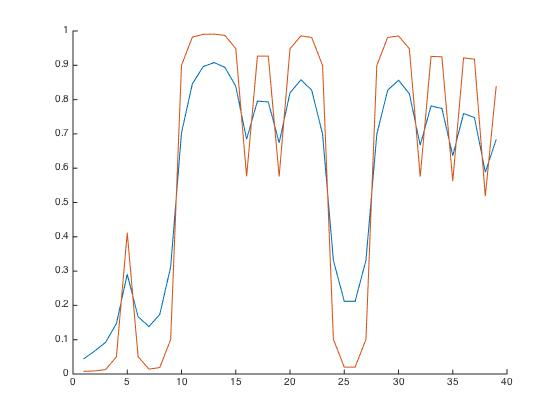
\includegraphics[width=5in]{output.jpg}
\caption{Distance versus node distribution}
\end{center}
\end{figure}
\paragraph{Algorithm :} 
 In order to get the above probability, we used forward backward algorithm to find joint probability. As the values get very small in a sequence , we used log form of probability and used log-sum trick to avoid the under flow.
 Once we get the joint probability, we divide that by p(x) by summing the $\alpha $ values for 39th week. \\ [.25cm]
 
 For this part , I got the probability that the economy is in a good state in the week of week 39 as $0.6830$
\subsubsection*{(b) Repeat (a) for $q = 0.9$, and compare the result to that of (a). Explain your comparison in one or two sentences. [15 pts]}
 For this part , I got the probability that the economy is in a good state in the week of week 39 as $0.8379$. From the graph, it can be seen, that higher emission means that output is more influenced by state. Thus, when state is $-1$, then $.9$ emission goes faster(more biased) towards bad state, similarly  state is $1$, then $.9$ emission goes faster(more biased) towards good state .

\end{document}
